\documentclass[12pt,letterpaper,twoside]{article}
\usepackage[utf8]{inputenc}
\usepackage[francais]{babel}
\usepackage[T1]{fontenc}
\usepackage{fullpage}
\usepackage{amsmath}
\usepackage{amsfonts}
\usepackage{amssymb}
\usepackage{pdfpages}
\usepackage{setspace}
\usepackage{float}
\usepackage{hyperref}
\usepackage{color}
\usepackage{multirow}
\usepackage{tabularx}
\usepackage{listings}

\onehalfspacing
\begin{document}

\setcounter{secnumdepth}{0}
\begin{titlepage}

        \vspace*{1cm}
        \begin{small}
        \begin{tabularx}{\textwidth}{ l X r }
        \multirow{3}{*}{
\includegraphics[height=1.5cm,keepaspectratio]{ul_logo.pdf}}
        && \'Equipe IA\\
        && Projet Robocup\\
        && Été 2016\\

        \scriptsize{\textbf{FACULTÉ DES SCIENCES ET GÉNIE}} && Robocup
        \end{tabularx}
        \end{small}

        \vfill

        \begin{center}

        Gestion de projet Robocup

        \vspace{0.5cm}

        Rencontre avec Beenox

        \vspace{2cm}

        \end{center}

        \vfill

        Date: 29 avril 2016

        \vspace{0.4cm}

        \rule{\textwidth}{2pt}

        \vspace{0.3cm}

        \begin{tabularx}{\textwidth}{ l X r }

        \textbf{Robocup} && \textbf{\'Equipe IA} \\

        \end{tabularx}


\end{titlepage}


\section*{Rencontre avec Beenox, 29 avril 2016}

\subsection*{Organisation du premier sprint de l'été 2016}
Les membres de Beenox nous ont donné quelques recommandations pour le sprint de cet été.
\begin{itemize}
\item \textbf{Temps de sprint maximal: 2 ou 3 semaines}
\item \textbf{Trouver un client et définir une date de fin précise}.
Plut\^ot que de définir une date arbitraire, trouver un <<client>>, par exemple un professeur, \`a qui l'on pourrait montrer notre progr\`es régulièrement.
\item \textbf{Si la tâche n'est pas écrite, elle ne sera pas faite.}
\item Avoir à la fin de chaque sprint un \textbf{<<sprint review>>}.
On peut ainsi mieux évaluer nos estimations de temps pour le prochain sprint.
\end{itemize}
Les membres de Beenox nous ont aussi proposé de mettre les tâches de notre sprint sur Slack, pour qu'ils puissent l'évaluer.

\subsection*{Intégration dans STA des outils crées pour la compétition}
Avoir un code standardisé est important pour l'intégration propre dans STA des outils.
Un code non standardisé doit \^etre considéré comme un code non fonctionnel/non livrable.
Cela sera traité avec les fork/pull request de \textit{GitHub}.
\\
Pour établir le standard du code, il vaut mieux de prendre comme base \textbf{un standard de code pré-établie} plut\^ot que d'en créer un `a partir de rien.

\subsection*{Probl\`emes de performances avec l'engin de compétition}
L'engin va avoir un temps global pour tous les systèmes.
On peut donc augmenter la performance en attendant un temps prédéfini avant de mettre à jour dans la <<Game Loop>> les données de chaque robot.

\begin{lstlisting}[language = python]
float time
if time > x
	#mettre a jour les donnees
\end{lstlisting}

\subsection*{Abstraction du niveau des stratégies}
La figure \ref{fig:gpo} représente les couches d'abstractions du \textit{Goal Oriented Programming}.
Chaque couche communique avec celle directement en bas et celle directement en haut.

\begin{figure}[htp]
\label{fig:gpo}
\centering
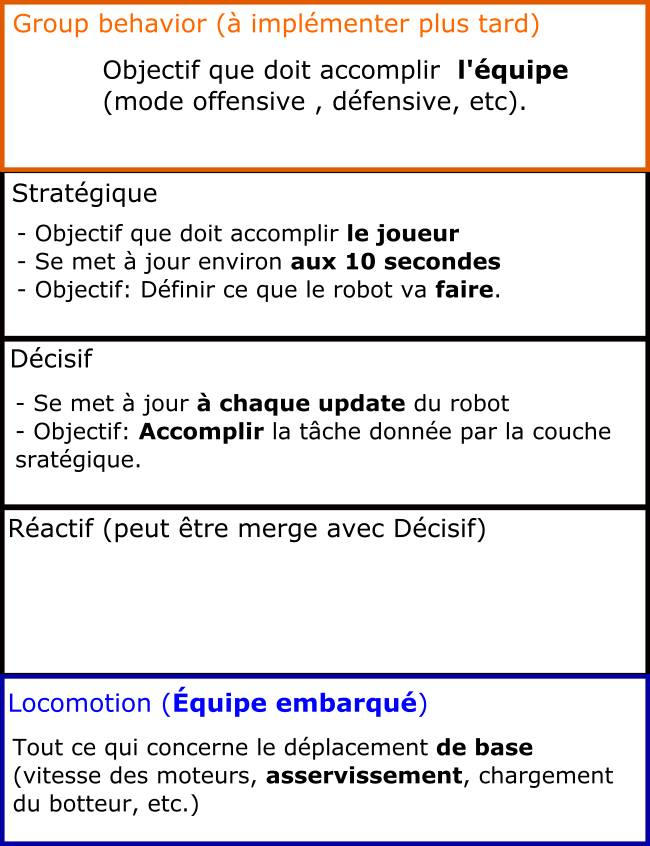
\includegraphics[height=9cm,keepaspectratio]{gpo_couches.png}
\caption{Couches d'abstractions du \textit{Goal Oriented Programming}}
\end{figure}

Il a aussi été recommandé de mettre l'emphase sur le développement des couches <<Tactique>> et <<Action>> de la STA.

\subsection*{Intégration des nouveaux}
Pour faciliter l'intégration des nouveaux, il faudrait avoir:
\begin{itemize}
\item Un wiki GitHub pour la documentation
\item Un << How to >> incluant:
\begin{itemize}
\item \textbf{Un guide d'installation}.
Il faut que n'importe qui puisse suivre les instructions et avoir une simulation de jeux sur son ordinateur sans problèmes.
\item \textbf{Les personnes ressources avec photo} pour chaque guide rédigé.
\end{itemize}
\end{itemize}

\subsection*{Références}
Alexandre Bergeron nous a envoyé une liste de livres et de sites que l'équipe pourra utiliser comme référence sur l'intelligence artificielle.

Il a aussi donné quelques recommandations par rapport au sujet:
\begin{itemize}
\item Les livres sur l'intelligence artificielle ont été rédigés avec les contraintes du jeu vidéo.
Nous n'avons pas ce genre de contraintes et pouvons éviter certaines abstractions difficiles.
\item Un vieux livre n'est pas nécessairement mauvais/dépassé.
\end{itemize}

\subsection*{Debug dans les jeux vidéo}
\begin{itemize}
\item Mettre \textbf{le plus d'information possible}.
\item L'interface doit être \textbf{facile à utiliser}.
\item De préférence, le débogueur doit être \textbf{toujours allumé}.
Un bogue peut être rare et difficile à reproduire.
\item Avoir un mode \textbf{image par image}.
Cela peut être produit avec une prise d'image à chaque intervalle de temps <<x>>.
\item Utiliser \textbf{le plus de possible log}.
De préférence, chaque robot a son log.
Dans ceux-ci, il  que au minimum:
\begin{itemize}
\item La \textbf{tactique} que le joueur exécute en ce moment.
\item L'\textbf{Action} que le joueur exécute en ce moment.
\end{itemize}

\end{itemize}

\subsection*{Autres conseils}
Notre système d'exploitation \textbf{n'est pas à temps réel}.
Il faut le considérer lors de l'écriture de code sensible au temps.

\subsection*{Membres présents}
\begin{itemize}
\item Ryma H.
\item Alexandre G.
\item Alexandra M.
\item Maxime G.
\item Maxime M.
\end{itemize}

\end{document}
